\begin{figure}[!ht]
    \centering
    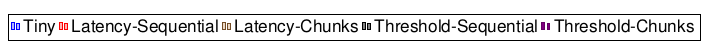
\includegraphics[scale=0.3]{images/legend}
    
    \subfloat[Tempo de execução]{
        \label{Labyrinth}
        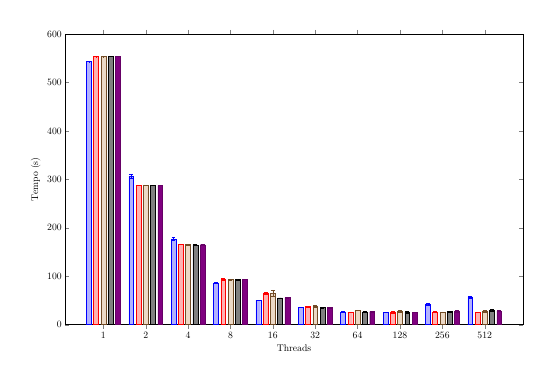
\begin{tikzpicture}[scale=0.35, baseline]
            \begin{axis}[
                width=1.5 \linewidth,
                height=1 \linewidth,
                %media de tempo intruder
                ybar=2.5pt,
                %enlargelimits=0.10,
                % legend style={at={(0.45,1.1)}, anchor=south, legend columns=-1},
                ylabel=Tempo (s),
                xlabel=Threads,
                symbolic x coords={1, 2, 4, 8, 16, 32, 64, 128, 256, 512},
                xtick=data,
                ymin=0,
                ymax=600,
                bar width=5pt,
                % nodes near coords,
                nodes near coords align={vertical},
            ]
            \addplot+[error bars,y dir=both, y explicit] coordinates {
                (1,543.12)+-(1,0.14) (2,307.12)+-(2,3.77) (4,177.18)+-(4,3.79) (8,86.06)+-(8,0.82) (16,50.63)+-(16,0.60) (32,35.89)+-(32,0.53) (64,26.45)+-(64,0.63) (128,25.83)+-(128,0.64) (256,41.98)+-(256,1.85) (512,57.32)+-(512,2.08) 
            };
            \addplot+[error bars,y dir=both, y explicit] coordinates {
                (1,553.57)+-(1,0.26) (2,287.70)+-(2,0.17) (4,165.86)+-(4,0.67) (8,94.13)+-(8,1.50) (16,65.04)+-(16,2.20) (32,37.22)+-(32,1.17) (64,25.60)+-(64,1.00) (128,25.49)+-(128,1.49) (256,26.10)+-(256,1.15) (512,25.80)+-(512,0.75)
            };
            \addplot+[error bars,y dir=both, y explicit] coordinates {
                (1,553.49)+-(1,0.21)(2,287.57)+-(2,0.25)(4,165.74)+-(4,0.99)(8,93.35)+-(8,1.29)(16,65.67)+-(16,6.11)(32,38.25)+-(32,1.76)(64,29.61)+-(64,0.77)(128,26.85)+-(128,2.24)(256,25.63)+-(256,0.42)(512,27.96)+-(512,1.35)
            };
            \addplot+[error bars,y dir=both, y explicit] coordinates {
                (1,553.89)+-(1,0.08) (2,287.30)+-(2,0.32) (4,164.88)+-(4,0.69) (8,93.33)+-(8,0.76) (16,55.06)+-(16,0.46) (32,35.27)+-(32,0.97) (64,26.35)+-(64,1.17) (128,26.33)+-(128,1.74) (256,26.96)+-(256,1.43) (512,29.70)+-(512,2.27) 
            };
            \addplot+[error bars,y dir=both, y explicit] coordinates {
                (1,553.38)+-(1,0.02) (2,287.58)+-(2,0.22) (4,164.99)+-(4,0.38) (8,93.83)+-(8,0.15) (16,55.92)+-(16,0.76) (32,35.17)+-(32,0.71) (64,26.79)+-(64,0.74) (128,25.67)+-(128,0.66) (256,27.99)+-(256,1.60) (512,28.01)+-(512,0.74)
            };
        % \legend {Tiny, Latency-Sequential, Latency-Chunks, Threshold-Sequential, Threshold-Chunks}
        \end{axis}
        \end{tikzpicture}
    }
    \subfloat[Aborts]{
        \label{abortLabyrinth}
        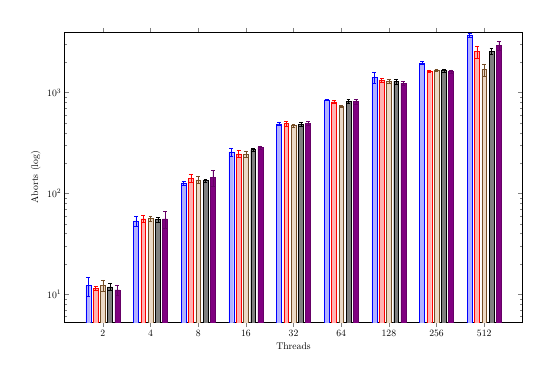
\begin{tikzpicture}[scale=0.35, baseline]
        \begin{axis}[
            ymode=log,
            width=1.5 \linewidth,
            height=1 \linewidth,
            %media de tempo intruder
            ybar=2.5pt,
            %enlargelimits=0.10,
            % legend style={at={(0.45,1.1)}, anchor=south, legend columns=-1},
            ylabel=Aborts (log),
            xlabel=Threads,
            symbolic x coords={1, 2, 4, 8, 16, 32, 64, 128, 256, 512},
            xtick=data,
            ymin=0,
            ymax=4000,
            bar width=5pt,
            % nodes near coords,
            nodes near coords align={vertical},
        ]
        \addplot+[error bars,y dir=both, y explicit] coordinates {
            (1,0.0)+-(1,0.0) (2,12.2)+-(2,2.63) (4,53.2)+-(4,5.94) (8,127.2)+-(8,6.14) (16,258.0)+-(16,24.04) (32,490.2)+-(32,16.41) (64,847.0)+-(64,12.39) (128,1413.4)+-(128,186.85) (256,1959.6)+-(256,67.08) (512,3727.2)+-(512,167.11) 
        };
        \addplot+[error bars,y dir=both, y explicit] coordinates {
            (1,0.0)+-(1,0.0) (2,11.4)+-(2,0.48) (4,56.0)+-(4,4.09) (8,142.0)+-(8,12.85) (16,245.8)+-(16,19.87) (32,491.2)+-(32,25.11) (64,811.8)+-(64,28.18) (128,1334.2)+-(128,63.09) (256,1633.4)+-(256,41.57) (512,2556.6)+-(512,340.72)
        };
        \addplot+[error bars,y dir=both, y explicit] coordinates {
             (1,0.0)+-(1,0.0) (2,12.2)+-(2,1.46) (4,56.4)+-(4,3.61) (8,136.4)+-(8,10.30) (16,245.4)+-(16,19.39) (32,473.2)+-(32,16.47) (64,734.8)+-(64,11.12) (128,1298.4)+-(128,60.09) (256,1677.2)+-(256,35.19) (512,1686.8)+-(512,244.04)
        };
        \addplot+[error bars,y dir=both, y explicit] coordinates {
            (1,0.0)+-(1,0.0) (2,11.8)+-(2,0.97) (4,54.8)+-(4,2.78) (8,134.8)+-(8,4.39) (16,271.2)+-(16,11.35) (32,482.8)+-(32,22.57) (64,822.0)+-(64,36.78) (128,1291.2)+-(128,74.59) (256,1657.8)+-(256,58.13) (512,2571.6)+-(512,174.36)
        };
        \addplot+[error bars,y dir=both, y explicit] coordinates {
            (1,0.0)+-(1,0.0) (2,11.0)+-(2,1.2) (4,55.72)+-(4,10.82) (8,143.2)+-(8,25.75) (16,286.0)+-(16,10.86) (32,496.6)+-(32,19.73) (64,812.0)+-(64,38.57) (128,1238.6)+-(128,53.69) (256,1629.6)+-(256,55.64) (512,2933.4)+-(512,289.46)
        };
        % \legend {Tiny, Latency-Sequential, Latency-Chunks, Threshold-Sequential, Threshold-Chunks}
        \end{axis}
        \end{tikzpicture}
    }
\end{figure}